% Options for packages loaded elsewhere
\PassOptionsToPackage{unicode}{hyperref}
\PassOptionsToPackage{hyphens}{url}
\documentclass[
]{article}
\usepackage{xcolor}
\usepackage{amsmath,amssymb}
\setcounter{secnumdepth}{-\maxdimen} % remove section numbering
\usepackage{iftex}
\ifPDFTeX
  \usepackage[T1]{fontenc}
  \usepackage[utf8]{inputenc}
  \usepackage{textcomp} % provide euro and other symbols
\else % if luatex or xetex
  \usepackage{unicode-math} % this also loads fontspec
  \defaultfontfeatures{Scale=MatchLowercase}
  \defaultfontfeatures[\rmfamily]{Ligatures=TeX,Scale=1}
\fi
\usepackage{lmodern}
\ifPDFTeX\else
  % xetex/luatex font selection
\fi
% Use upquote if available, for straight quotes in verbatim environments
\IfFileExists{upquote.sty}{\usepackage{upquote}}{}
\IfFileExists{microtype.sty}{% use microtype if available
  \usepackage[]{microtype}
  \UseMicrotypeSet[protrusion]{basicmath} % disable protrusion for tt fonts
}{}
\makeatletter
\@ifundefined{KOMAClassName}{% if non-KOMA class
  \IfFileExists{parskip.sty}{%
    \usepackage{parskip}
  }{% else
    \setlength{\parindent}{0pt}
    \setlength{\parskip}{6pt plus 2pt minus 1pt}}
}{% if KOMA class
  \KOMAoptions{parskip=half}}
\makeatother
\usepackage{graphicx}
\makeatletter
\newsavebox\pandoc@box
\newcommand*\pandocbounded[1]{% scales image to fit in text height/width
  \sbox\pandoc@box{#1}%
  \Gscale@div\@tempa{\textheight}{\dimexpr\ht\pandoc@box+\dp\pandoc@box\relax}%
  \Gscale@div\@tempb{\linewidth}{\wd\pandoc@box}%
  \ifdim\@tempb\p@<\@tempa\p@\let\@tempa\@tempb\fi% select the smaller of both
  \ifdim\@tempa\p@<\p@\scalebox{\@tempa}{\usebox\pandoc@box}%
  \else\usebox{\pandoc@box}%
  \fi%
}
% Set default figure placement to htbp
\def\fps@figure{htbp}
\makeatother
\setlength{\emergencystretch}{3em} % prevent overfull lines
\providecommand{\tightlist}{%
  \setlength{\itemsep}{0pt}\setlength{\parskip}{0pt}}
\usepackage{bookmark}
\IfFileExists{xurl.sty}{\usepackage{xurl}}{} % add URL line breaks if available
\urlstyle{same}
\hypersetup{
  hidelinks,
  pdfcreator={LaTeX via pandoc}}

\author{}
\date{}

\begin{document}

\section{Paper 8: Two Accountings --- Condensation, Internal Expansion,
and the Area
Law}\label{paper-8-two-accountings-condensation-internal-expansion-and-the-area-law}

\subsection{\texorpdfstring{Inversion of the Splitting Theorem under
Shared-Curvature Accounting, the Jeans-Type Threshold, the Internal
Clock and \(a\propto t^{1/2}\), and the Vacuum as a
Reservoir}{Inversion of the Splitting Theorem under Shared-Curvature Accounting, the Jeans-Type Threshold, the Internal Clock and a\textbackslash propto t\^{}\{1/2\}, and the Vacuum as a Reservoir}}\label{inversion-of-the-splitting-theorem-under-shared-curvature-accounting-the-jeans-type-threshold-the-internal-clock-and-apropto-t12-and-the-vacuum-as-a-reservoir}

Author: Noriaki Kihara\\
Affiliation: WF System Co., Ltd.\\
ORCID: 0009-0004-6753-4020\\
Version: v0.2\\
Date: June 2026\\
DOI (this version): 10.5281/zenodo.20640461\\
Concept DOI: 10.5281/zenodo.20640460\\
License: CC BY 4.0

\begin{center}\rule{0.5\linewidth}{0.5pt}\end{center}

\subsection{Abstract}\label{abstract}

The no-exception splitting theorem of Paper 5 was based on \textbf{local
accounting}, in which each fragment carries its own container, and its
conclusion was complete dispersal. The core of the present model,
however, is that \(R^2=\sum\nu^2\) sets a curvature-like scale, and
local accounting on a flat background is not consistent with the model's
own claim. This paper puts the curvature into the accounting and obtains
three results.

First, the \textbf{inversion of the splitting theorem}: when all
fragments ride on a single shared container determined self-consistently
by the total content \(S\), minimizing the unfilled amount becomes
equivalent to maximizing the total capacity, and an exhaustive check for
\(S\le25\) shows that \textbf{condensation (the single fragment) is
strictly optimal}. Local accounting (surface term \(s^{3/2}\),
subadditive) → dispersal; shared accounting (capacity term \(s^2\),
superadditive) → condensation --- the divide is a single exponent, and
physically it is the choice of whether the container = the curvature
belongs to each fragment or is shared. In a one-parameter family mixing
the two accountings, the condensation onset threshold behaves as
\(w^*(S)\approx 3.40/\sqrt S\to0\): \textbf{the larger the system, the
more a slight sharing of geometry suffices for condensation to dominate}
(a scaling of the same form as the Jeans criterion; a structural
correspondence, not an identification). Under the exclusion rule (Paper
7), the competitor on the dispersal side changes from the all-1
partition to a Fermi-sea-type configuration, so the threshold drops
further (\(0.6397\to0.5872\) at \(S=9\)).

Second, the \textbf{internal expansion law}: when the internal splitting
cascade of a closed state space (container fixed, no exterior) is read
through the ratios of an internal observer (who uses their own fragment
as the measuring rod and carries the dual clock \(\tau=1/R'\)), the
apparent scale factor satisfies the exact identity \(a^4 f=\pi^2/2\)
(\(f\) is the occupancy fraction) and, in the leading term, follows

\[
a\propto t^{1/2}
\]

(a universal law independent of the branching number; the fitted
exponent in the central window of a deep ternary cascade is 0.507).
\(f\propto a^{-4}\) is the 4-dimensional dilution of a conserved number,
and the appearance of a radiation-type dilution law in a system whose
content is oscillation only is a consistency check. Expansion requires
neither an exterior nor growth of the container: \textbf{a system that
subdivides inward looks expanding when measured with a measuring rod
that itself shrinks.} We give the numbers including the exclusion-rule
correction of the endpoint (the cascade terminates at \(s'=3\), and the
all-1 state is unreachable).

Third, the \textbf{area law and the reservoir}: the phase-space area per
state is a rigid body of exactly 2 (\(=4\delta_{\min}^2\)), and the
conservation of total area is the same law as the dual reading of energy
conservation. On the other hand, imposing exact conservation of mode
area freezes the cascade at stage 0. The exact conservation law that
actually holds is ``occupied area + gap = container volume,'' and
splitting is the process of transferring occupied area into the gap.
\textbf{The vacuum-like state (the gap) is not a structureless void but
a reservoir of area that makes evolution possible.}

\begin{center}\rule{0.5\linewidth}{0.5pt}\end{center}

\subsection{Keywords}\label{keywords}

condensation, dispersal, shared container, Jeans-type threshold,
internal observer, scale factor, radiation-type dilution, area law,
rigid tiling, reservoir, occupancy fraction

\begin{center}\rule{0.5\linewidth}{0.5pt}\end{center}

\subsection{1. Introduction}\label{introduction}

The classical insight into self-aggregation under gravity goes back to
the Jeans criterion {[}5{]}, by which the instability of a uniform
medium depends on scale (the larger the scale, the more gravity
dominates). Support by degeneracy pressure (Chandrasekhar {[}6{]}) is
the classical example of a structure in which exclusion statistics
opposes aggregation. The viewpoint that the accountings of geometry,
thermodynamics, and information are two sides of one ledger is
represented by Jacobson's thermodynamic derivation of spacetime {[}7{]}.

This paper does not extend these physical theories. What it does is to
establish, \textbf{inside the counting model}, by exhaustive checks and
exact identities, the following three points: (i) the choice of
accounting (local or shared) switches between dispersal and
condensation; (ii) an expansion-like power law appears in the reading of
an internal observer; and (iii) the area ledger requires vacuum-like
regions as a reservoir. All correspondences with standard cosmology (the
scale factor; the power law of the radiation-dominated era {[}8{]}) are
recorded as structural correspondences with alarms attached, and no
identification is made.

\begin{center}\rule{0.5\linewidth}{0.5pt}\end{center}

\subsection{2. Two Accountings and the Inversion of the Splitting
Theorem}\label{two-accountings-and-the-inversion-of-the-splitting-theorem}

\subsubsection{2.1 Local accounting
(review)}\label{local-accounting-review}

The splitting theorem of Paper 5 {[}2{]} is based on the local
accounting \(\Delta_{\mathrm{loc}}=\sum_a[V_4(R_a)-N_0(R_a)]\), in which
each fragment \(a\) carries its own circumscribing container
\(V_4(R_a)\). The leading term of the volume gap is the surface term
\(\propto s^{3/2}\), and by the subadditivity associated with the power
\(3/2>1\), consistent splitting reduces the gap without exception ---
the conclusion is complete dispersal.

\subsubsection{2.2 The shared container (global
accounting)}\label{the-shared-container-global-accounting}

In the present model (Paper 4 {[}1{]}), \(R^2=\sum\nu^2\) sets a
curvature-like scale (it can be written in the form
\(\Lambda_{\mathrm{model}}=3/R_c^2\)). We therefore let all fragments
ride on a single container \(S^4(R_c)\), \(R_c^2=S\), determined
self-consistently by the total content \(S=\sum_a s_a\). Under fixed
\(S\) the container volume is the same for every partition, so
minimizing the global mismatch is equivalent to \textbf{maximizing the
total capacity \(\sum_a N_0(\sqrt{s_a})\)} (by this equivalence the
conclusion does not depend on the choice of the container constant).

Results of the exhaustive check of consistent partitions for \(S\le25\):

\begin{enumerate}
\def\labelenumi{\arabic{enumi}.}
\tightlist
\item
  \textbf{Odd \(S\)}: the single fragment \((S)\) is, without exception,
  the unique optimum.
\item
  \textbf{Even \(S\)}: since no single slot exists, the optimum is
  always \((S-1,1)\) --- the largest fragment plus the minimal
  satellite. Not the symmetric partition but the \textbf{maximally
  asymmetric} one wins (an accretion-type ``rich get richer'' structure
  due to the convexity of the capacity).
\end{enumerate}

\begin{figure}
\centering
\pandocbounded{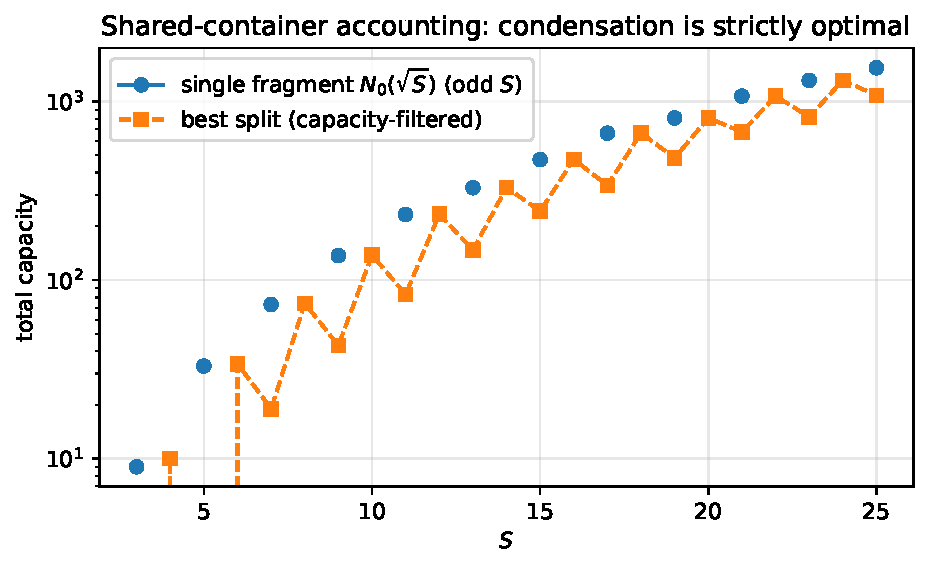
\includegraphics[keepaspectratio]{figure_paper8_1_condensation.pdf}}
\caption{Figure 1. Condensation optimality under the shared container}
\end{figure}

\textbf{Figure 1. Shared-container accounting (exhaustive for
\(S\le25\), with the capacity law included): the capacity of the single
fragment strictly exceeds that of every partition.}

\subsubsection{\texorpdfstring{2.3 Restriction of merger channels by the
\(Z_2\) selection
rule}{2.3 Restriction of merger channels by the Z\_2 selection rule}}\label{restriction-of-merger-channels-by-the-z_2-selection-rule}

Since consistent fragments carry odd labels, odd + odd = even has no
parent slot, and \textbf{two-body mergers are forbidden}. The minimal
allowed merger, once the exclusion rule (Paper 7 {[}4{]}, \(c(1)=1\)) is
included, is \((3,3,1)\to7\).

\subsubsection{2.4 The Jeans-type
threshold}\label{the-jeans-type-threshold}

By an exhaustive check of a one-parameter family in which the container
is mixed as ``local \((1-w)\) + shared \(w\)'', the condensation onset
threshold behaves as

\[
w^*(S)\;\approx\;\frac{32}{3\pi}\,S^{-1/2}\;\approx\;\frac{3.40}{\sqrt S}\;\longrightarrow\;0
\]

(the exact formula \(w^*=1-(N_0(\sqrt S)-S)/[\tfrac{\pi^2}2 S(S-1)]\)
has been checked against bisection). \textbf{The larger the scale, the
more the condensation side wins} --- a scaling of the same form as the
Jeans criterion {[}5{]}.

\begin{figure}
\centering
\pandocbounded{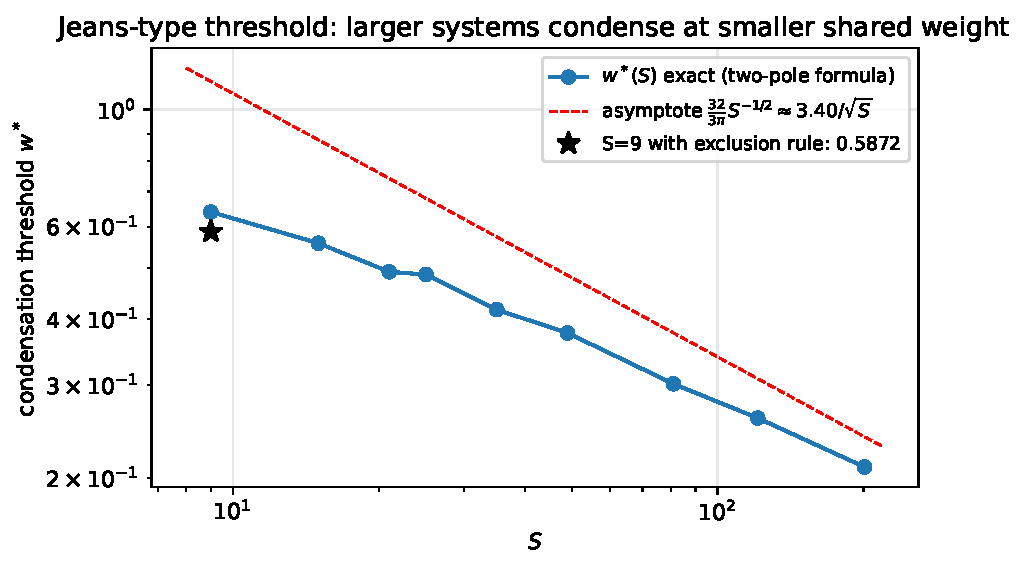
\includegraphics[keepaspectratio]{figure_paper8_2_jeans_threshold.pdf}}
\caption{Figure 2. Jeans-type condensation threshold}
\end{figure}

\textbf{Figure 2. The Jeans-type threshold \(w^*(S)\): the exact formula
and the asymptotic form \(3.40/\sqrt S\). The star marks the revised
value 0.5872 at \(S=9\) under the exclusion rule.}

\subsubsection{2.5 Revision by the exclusion
rule}\label{revision-by-the-exclusion-rule}

Under the capacity law of Paper 7, the maximal dispersal within a single
lattice is not the all-1 partition but the \textbf{Fermi-sea type}
(occupying one cell at a time from the lowest shell,
\(n_{\max}\approx\tfrac{\pi^2}2 M_F^2\sim S^{2/3}\),
\(M_F\approx(3S/\pi^2)^{1/3}\)). Since the competitor on the dispersal
side is weakened, the condensation threshold drops: at \(S=9\),
\(w^*=0.6397\to0.5872\). It is worth noting that exclusion statistics
appears on the dispersal side as a degeneracy-pressure-type structure
(of the same form as Chandrasekhar {[}6{]}; a structural
correspondence).

\subsubsection{2.6 Two attractors of the occupancy
fraction}\label{two-attractors-of-the-occupancy-fraction}

On the self-consistent container, the occupancy fraction is
\(f_{\mathrm{disp}}\approx0.0848\,S^{-4/3}\propto\Lambda_{\mathrm{model}}^{4/3}\)
in the dispersed state (Fermi sea, the revised value including the
exclusion rule) and \(f_{\mathrm{cond}}\to3/16\) (a universal value) in
the condensed state. The two-phase coexistence of a dilute global
background and packed local clumps is recorded as a qualitative
observation (the mapping to observables is quarantined in the appendix
with alarms attached).

\begin{center}\rule{0.5\linewidth}{0.5pt}\end{center}

\subsection{\texorpdfstring{3. The Internal Expansion Law:
\(a\propto t^{1/2}\)}{3. The Internal Expansion Law: a\textbackslash propto t\^{}\{1/2\}}}\label{the-internal-expansion-law-apropto-t12}

\subsubsection{3.1 Setup}\label{setup}

Consider the internal splitting cascade of a closed state space
(\(R_c^2=S\) fixed, no exterior). When the fragments carry a
representative value \(s'\) and there are \(n=S/s'\) of them, defining
the apparent scale factor as the ratio of the mean inter-fragment
distance to the fragment size, \(a=d/R'\), it satisfies with the
occupancy fraction the exact identity, in the leading term,

\[
a^4\,f=\frac{\pi^2}{2}.
\]

\textbf{Apparent expansion and rarefaction are two readings of one and
the same quantity}, and \(f\propto a^{-4}\) has the same form as the
dilution of a conserved number in 4 dimensions (radiation type).

\subsubsection{3.2 The internal clock and the main
result}\label{the-internal-clock-and-the-main-result}

The proper period of each fragment is \(\tau=1/R'=\lambda'\) ---
\textbf{the dual relation \(\nu\lambda=1\) is itself the clock} (Paper 6
{[}3{]}). The \(Z_2\) selection rule forbids binary trees, so the
minimal cascade is the ternary tree. For a \(k\)-ary self-similar
cascade:

\begin{itemize}
\tightlist
\item
  With respect to the stage number: the e-folds per stage are
  \(\ln k/4\) (exponential growth).
\item
  \textbf{With respect to internal time}: from \(a^4\propto1/s'\) and
  \(t\propto1/\sqrt{s'}\), in the leading term
\end{itemize}

\[
\boxed{\;a\propto t^{1/2}\;}
\]

\textbf{independent of the branching number \(k\)} (it holds for an
arbitrary geometric schedule). The fitted exponent in the central window
of a deep ternary cascade (\(S=3^{14}\)) is 0.507.

\subsubsection{3.3 The radiation law as a consistency
check}\label{the-radiation-law-as-a-consistency-check}

\(f\propto a^{-4}\) is the dilution law of radiation, and the content of
this model is \(\nu\) (oscillation) only. \textbf{That the radiation-era
law appears is the correct answer; a matter-era or constant-term-era law
would have been a contradiction.} This is not a fit but a consistency
check (the correspondence with cosmology is a structural correspondence
{[}8{]}).

\subsubsection{3.4 The endpoint correction by the exclusion rule and the
specificity of the
clock}\label{the-endpoint-correction-by-the-exclusion-rule-and-the-specificity-of-the-clock}

By the capacity law the final stage \(3\to(1,1,1)\) is forbidden, and
\textbf{the cascade terminates at \(s'=3\)} (the total number of e-folds
is \(\tfrac14\ln(S/3)+\tfrac14\ln(\pi^2/2)\)). The endpoint correction
factor remains, by the coincidence \(N_0(\sqrt3)=9=3^2\), exactly
\(\pi^2/2\), unchanged.

We also checked robustness with respect to the choice of clock:
\(a\propto t^{1/2}\) is a law \textbf{specific to the dual clock}. With
the area clock (cumulative released area), time saturates at a ceiling
and no power law appears; with the stage clock, the law is exponential.
The precise status is: ``the radiation-era law when \(\nu\lambda=1\) is
chosen as the clock.''

\begin{figure}
\centering
\pandocbounded{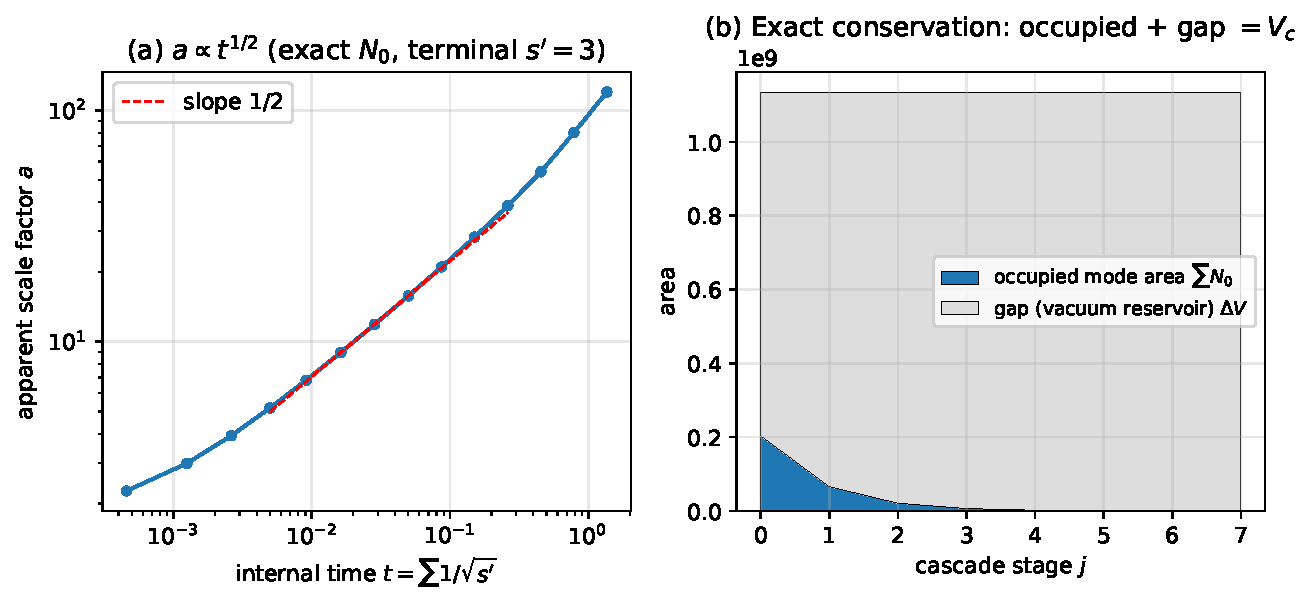
\includegraphics[keepaspectratio]{figure_paper8_3_expansion_reservoir.pdf}}
\caption{Figure 3. Internal expansion law and the vacuum reservoir}
\end{figure}

\textbf{Figure 3. (a) The internal expansion law \(a\propto t^{1/2}\)
(exact \(N_0\), termination at \(s'=3\)). (b) The exact conservation
law: occupied area + gap = container volume (the vacuum = the
reservoir).}

\subsubsection{3.5 Interpretive implications (within the model,
restricted)}\label{interpretive-implications-within-the-model-restricted}

\begin{enumerate}
\def\labelenumi{(\roman{enumi})}
\tightlist
\item
  Expansion requires neither an exterior nor growth of the container ---
  expansion is another name for the subdivision of the measuring rod.
  (ii) Regions that appear mutually distant are, when the hierarchy is
  traced back, internal subdivisions of the same parent cell, so no
  separate assumption of initial causal contact is required (an
  observation within the model; it does not claim to solve the horizon
  problem). (iii) The ``beginning'' can be read, without any explosion,
  as the onset of the splitting cascade from an undifferentiated single
  cell of the highest frequency.
\end{enumerate}

\begin{center}\rule{0.5\linewidth}{0.5pt}\end{center}

\subsection{4. The Area Law and the Vacuum as a
Reservoir}\label{the-area-law-and-the-vacuum-as-a-reservoir}

\subsubsection{4.1 Rigid tiling}\label{rigid-tiling}

The jumps of \(N_0(\sqrt s)\) occur only at odd \(s\), and each
consistent label \(m\) owns a window \([m,m+2)\) of width exactly 2 on
the \(s\) axis. The area per state,

\[
\Delta s=2=4\,\delta_{\min}^2,
\]

is a \textbf{rigid body} (upper bound = lower bound), and the
conservation of total area \(\sum\delta_a^2=S/2\) is the same law as the
dual reading of energy conservation \(\sum\nu_a^2=S\). The logarithmic
area and the \((\nu,\lambda)\) area agree exactly on the constraint
(Jacobian \(1/\nu\lambda=1\)), and the necessary and sufficient
condition for splitting to be realizable as an area-preserving map
(piecewise symplectic) is the summability of the areas (a Moser-type
existence theorem).

\subsubsection{4.2 Strong conservation freezes
evolution}\label{strong-conservation-freezes-evolution}

If area is read as the mode number \(\sum N_0\) and exact conservation
without a reservoir is imposed, then in every consistent partition with
\(s\le25\) the mode area decreases without exception (the strict
superadditivity of \(N_0\)). Hence \textbf{under an area conservation
law without a reservoir, the cascade freezes at stage 0}.

\subsubsection{4.3 The true conservation law and the
reservoir}\label{the-true-conservation-law-and-the-reservoir}

The exact conservation law that actually holds is

\[
\text{occupied area}\ \textstyle\sum N_0\;+\;\text{gap}\ \Delta V\;=\;V_c\;=\;\text{constant}
\]

(verified to hold identically at every stage of the ternary cascade).
Splitting is the process of transferring occupied mode area into the
gap, and the release is front-loaded (the first splitting releases the
fraction \(1-1/k\) of the capacity).

\begin{quote}
\textbf{The vacuum-like state (the gap) is not a structureless void but
a reservoir of area that makes evolution possible.} Condensation (§2)
can be read as the withdrawal of area from this reservoir (the reverse
process).
\end{quote}

\begin{center}\rule{0.5\linewidth}{0.5pt}\end{center}

\subsection{5. Scope of Claims of This
Paper}\label{scope-of-claims-of-this-paper}

What this paper claims: (1) The optimality of condensation under shared
accounting (exhaustive check) and the local/shared divide by a single
exponent. (2) The restriction of merger channels by \(Z_2\) and the
exclusion rule. (3) The Jeans-type threshold \(w^*\propto S^{-1/2}\)
(with the exact formula). (4) The identity \(a^4f=\pi^2/2\) and
\(a\propto t^{1/2}\) (specific to the dual clock, independent of the
branching number, with the endpoint correction included). (5) Rigid
tiling; area conservation = the dual reading of energy conservation;
occupied + gap = constant; and the reservoir structure.

What this paper does not claim: (1) A derivation of gravity, cosmic
expansion, or vacuum energy (``condensation,'' ``expansion,'' and
``vacuum'' are descriptions of configuration comparisons and counting
ratios within the model). (2) A force as a function of distance (what
this paper exhibits is a configuration preference, not a force; for the
quantification of position on the \(\lambda\) side, the relational
geometry of Paper 7 is the first step). (3) A within-model derivation of
the mixing parameter \(w\). (4) An explanation of the numbers of
observational cosmology (the mapping in the appendix is a record with
alarms attached and has no independent support).

\begin{center}\rule{0.5\linewidth}{0.5pt}\end{center}

\subsection{6. Conclusion}\label{conclusion}

A single choice of accounting --- whether the container = the curvature
belongs to each fragment or is shared --- switches between dispersal and
condensation. Shared curvature gives condensation; internal splitting
gives the expansion-like power law \(a\propto t^{1/2}\); and the area
ledger gives the vacuum as a reservoir --- each with no additional
mechanism. The model has both the dispersing tendency and the condensing
tendency built in, and the divide of their competition is quantified as
a scale-dependent threshold.

The central observation of this paper is that the three aspects ---
``the coexistence of a dilute global background and condensed local
clumps,'' ``the radiation-type dilution law,'' and ``the vacuum as the
fuel of evolution'' --- emerge from nothing but the inventory of
\(\nu\lambda=1\), the zeros, and the asymmetric one bit.

\begin{center}\rule{0.5\linewidth}{0.5pt}\end{center}

\subsection{Appendix A: Mapping to Observables (a Record with Alarms
Attached)}\label{appendix-a-mapping-to-observables-a-record-with-alarms-attached}

Substituting the observed occupancy fraction
\(f_{\mathrm{obs}}\sim1.6\times10^{-31}\) (the nondimensionalization of
0.25 hydrogen atoms per m³) into the identity for the dispersed state
gives \(S\approx2\times10^{22}\), and the scale width of a single
hierarchy level is about 11 orders of magnitude, which does not reach
the observed scale width (36--61 orders of magnitude). \textbf{The
single-hierarchy mapping is rejected} (recorded as a sound negative
result). The cross-check for the case where nesting of hierarchy levels
multiplies the widths has not been carried out, and the recovery of
testability requires an independent third dimensionless observable.

\subsection{Appendix B: Essentials of the Reproduction
Procedure}\label{appendix-b-essentials-of-the-reproduction-procedure}

By the full enumeration of consistent partitions (\(S\le25\)), bisection
for the mixed accounting (40 iterations), the cascade tables
(\(k=3,m=14\), exact \(N_0\)), the tiling check (\(s\le40\)), and the
verification of the reservoir identity at every stage. The scripts and
research notes are provided in the public repository
(https://github.com/WurabeSeiji/ai-chat-logs-open).

\begin{center}\rule{0.5\linewidth}{0.5pt}\end{center}

\subsection{References}\label{references}

{[}1{]} Noriaki Kihara, Paper 4, v1.0, 2026. Concept DOI:
10.5281/zenodo.20638962.

{[}2{]} Noriaki Kihara, Paper 5, v0.2, 2026. Concept DOI: 10.5281/zenodo.20640454.

{[}3{]} Noriaki Kihara, Paper 6, v0.2, 2026. Concept DOI: 10.5281/zenodo.20640456.

{[}4{]} Noriaki Kihara, Paper 7, v0.2, 2026. Concept DOI: 10.5281/zenodo.20640458.

{[}5{]} J. H. Jeans, ``The stability of a spherical nebula,''
Philosophical Transactions of the Royal Society A 199 (1902), 1--53.

{[}6{]} S. Chandrasekhar, \emph{An Introduction to the Study of Stellar
Structure}, University of Chicago Press, 1939.

{[}7{]} T. Jacobson, ``Thermodynamics of spacetime: The Einstein
equation of state,'' Physical Review Letters 75 (1995), 1260--1263.

{[}8{]} S. Weinberg, \emph{Cosmology}, Oxford University Press, 2008.

\begin{center}\rule{0.5\linewidth}{0.5pt}\end{center}

\subsection{License}\label{license}

This paper is published under CC BY 4.0.\\
Reuse, adaptation, translation, and citation are permitted, provided
that the author name, version, publication date, and source are clearly
indicated.

\end{document}
